\documentclass[margin=2mm]{standalone}
\usepackage{tikz}
\begin{document}
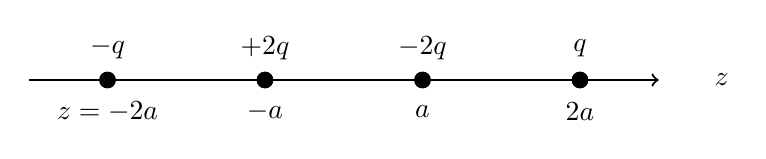
\begin{tikzpicture}
    \draw [->, thick] (0,0) -- (8,0) node[near end, pos=1.1] {$z$};
    \foreach \x in {1, 3, 5, 7}
        \draw [fill] (\x,0) circle (0.1);
    
    \node at (1, 0.4) {$-q$};
    \node at (3, 0.4) {$+2q$};
    \node at (5, 0.4) {$-2q$};
    \node at (7, 0.4) {$q$};
    \node at (1, -0.4) {$z=-2a$};
    \node at (3, -0.4) {$-a$};
    \node at (5, -0.4) {$a$};
    \node at (7, -0.4) {$2a$};
\end{tikzpicture}
\end{document}